\documentclass[11pt]{article}
\usepackage[utf8]{inputenc}
\usepackage[T1]{fontenc}
\usepackage{lmodern}
\usepackage{geometry}
\usepackage{tikz}
\usetikzlibrary{arrows.meta,shapes.geometric}

\geometry{paperwidth=16cm,paperheight=6.2cm,margin=0cm}
\pagestyle{empty}
\setlength{\parindent}{0pt}

\definecolor{ctxFill}{RGB}{238,242,245}
\definecolor{ctxLine}{RGB}{155,168,179}
\definecolor{ctxText}{RGB}{38,52,67}
\definecolor{exFill}{RGB}{220,233,247}
\definecolor{exLine}{RGB}{23,54,93}
\definecolor{prFill}{RGB}{200,240,236}
\definecolor{prLine}{RGB}{8,127,140}
\definecolor{prText}{RGB}{6,79,87}
\definecolor{phFill}{RGB}{234,242,245}

\begin{document}
\noindent
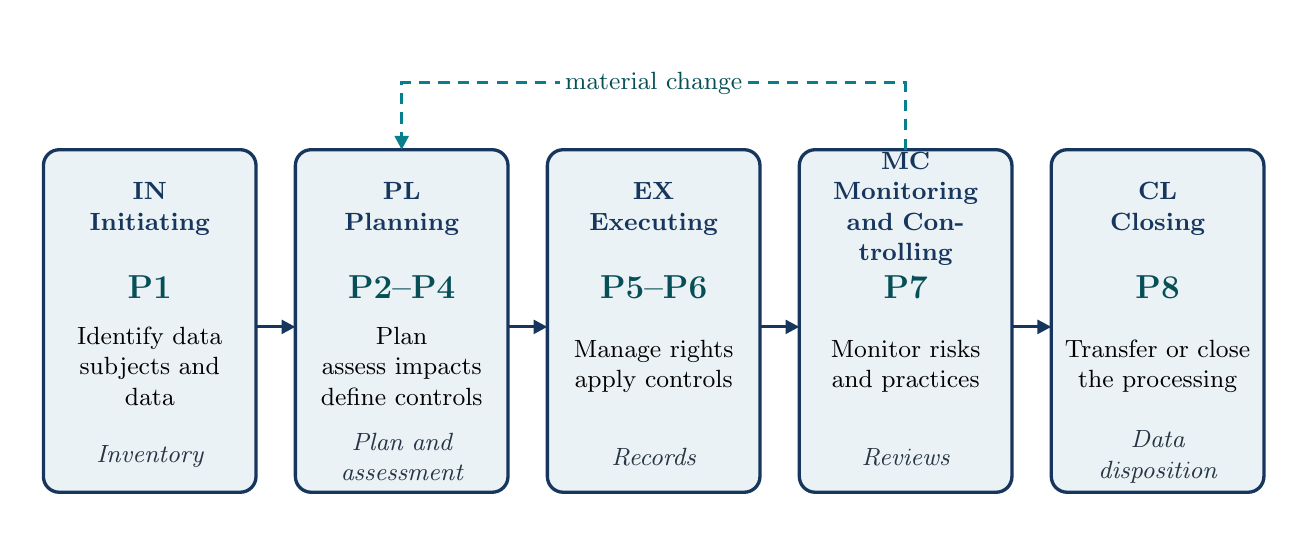
\begin{tikzpicture}[x=1cm,y=1cm,font=\small]
  \path[use as bounding box] (0,0) rectangle (16,6.2);
  \draw[fill=phFill,draw=exLine,line width=1.2pt,rounded corners=0.2cm] (0.2,0.3) rectangle (2.9000000000000004,4.65);
  \node[align=center,text width=2.5cm,text=exLine] at (1.55,3.9) {\small\bfseries IN\\Initiating};
  \node[align=center,text=prText] at (1.55,2.9) {\large\textbf{P1}};
  \node[align=center,text width=2.5cm] at (1.55,1.9) {\small Identify data\\subjects and\\data};
  \node[align=center,text width=2.5cm,text=ctxText] at (1.55,0.75) {\small\itshape Inventory};
  \draw[draw=exLine,line width=1.1pt,-{Triangle[length=5pt,width=5pt]}] (2.9000000000000004,2.4) -- (3.4000000000000004,2.4);
  \draw[fill=phFill,draw=exLine,line width=1.2pt,rounded corners=0.2cm] (3.4000000000000004,0.3) rectangle (6.1000000000000005,4.65);
  \node[align=center,text width=2.5cm,text=exLine] at (4.75,3.9) {\small\bfseries PL\\Planning};
  \node[align=center,text=prText] at (4.75,2.9) {\large\textbf{P2–P4}};
  \node[align=center,text width=2.5cm] at (4.75,1.9) {\small Plan\\assess impacts\\define controls};
  \node[align=center,text width=2.5cm,text=ctxText] at (4.75,0.75) {\small\itshape Plan and\\assessment};
  \draw[draw=exLine,line width=1.1pt,-{Triangle[length=5pt,width=5pt]}] (6.1000000000000005,2.4) -- (6.6000000000000005,2.4);
  \draw[fill=phFill,draw=exLine,line width=1.2pt,rounded corners=0.2cm] (6.6000000000000005,0.3) rectangle (9.3,4.65);
  \node[align=center,text width=2.5cm,text=exLine] at (7.950000000000001,3.9) {\small\bfseries EX\\Executing};
  \node[align=center,text=prText] at (7.950000000000001,2.9) {\large\textbf{P5–P6}};
  \node[align=center,text width=2.5cm] at (7.950000000000001,1.9) {\small Manage rights\\apply controls};
  \node[align=center,text width=2.5cm,text=ctxText] at (7.950000000000001,0.75) {\small\itshape Records};
  \draw[draw=exLine,line width=1.1pt,-{Triangle[length=5pt,width=5pt]}] (9.3,2.4) -- (9.8,2.4);
  \draw[fill=phFill,draw=exLine,line width=1.2pt,rounded corners=0.2cm] (9.8,0.3) rectangle (12.5,4.65);
  \node[align=center,text width=2.5cm,text=exLine] at (11.15,3.9) {\small\bfseries MC\\Monitoring\\and Controlling};
  \node[align=center,text=prText] at (11.15,2.9) {\large\textbf{P7}};
  \node[align=center,text width=2.5cm] at (11.15,1.9) {\small Monitor risks\\and practices};
  \node[align=center,text width=2.5cm,text=ctxText] at (11.15,0.75) {\small\itshape Reviews};
  \draw[draw=exLine,line width=1.1pt,-{Triangle[length=5pt,width=5pt]}] (12.5,2.4) -- (13.0,2.4);
  \draw[fill=phFill,draw=exLine,line width=1.2pt,rounded corners=0.2cm] (13.0,0.3) rectangle (15.7,4.65);
  \node[align=center,text width=2.5cm,text=exLine] at (14.35,3.9) {\small\bfseries CL\\Closing};
  \node[align=center,text=prText] at (14.35,2.9) {\large\textbf{P8}};
  \node[align=center,text width=2.5cm] at (14.35,1.9) {\small Transfer or close\\the processing};
  \node[align=center,text width=2.5cm,text=ctxText] at (14.35,0.75) {\small\itshape Data\\disposition};
  \draw[draw=prLine,line width=1.1pt,dash pattern=on 4pt off 3pt,-{Triangle[length=5pt,width=5pt]}] (11.15,4.65) -- (11.15,5.5) -- (4.75,5.5) -- (4.75,4.65);
  \node[text=prText,fill=white,inner sep=2pt] at (7.95,5.5) {\small material change};
\end{tikzpicture}
\end{document}
